\documentclass{article}
\usepackage{graphicx}
\usepackage{amsmath,amsthm,amssymb}
\usepackage[font=small,labelfont=bf]{caption}
\usepackage{tikz}
\usetikzlibrary{calc, angles, quotes, shapes.geometric}
\usepackage{tkz-euclide}
\usepackage{float}
\usepackage[margin=1in]{geometry}
\usepackage{gensymb}
\usepackage{hyperref}
\hypersetup{
    colorlinks=true,
    linkcolor=blue,
    filecolor=magenta,      
    urlcolor=cyan,
    pdftitle={Overleaf Example},
    pdfpagemode=FullScreen,
    }
\usepackage{fancyhdr}
\pagestyle{fancy}
\fancyhead[R]{Enoch Yu}
\pagenumbering{gobble}
\usepackage{enumitem}
\newtheorem{theorem}{Theorem}[section]
\newtheorem{lemma}[theorem]{Lemma}
\newtheorem*{lemma*}{Lemma}
\newtheorem{sublemma}{Lemma}[section]
\newtheorem{proposition}{Proposition}
\newtheorem{corollary}{Corollary}[theorem]
\newenvironment{solution}{\begin{trivlist}\item[]{\bf Solution}}{\qed \end{trivlist}}
\newcommand{\verteq}{\rotatebox{90}{$\;\;=\;\;$}}
\newcommand*\circled[1]{\tikz[baseline=(char.base)]{
            \node[shape=circle,draw,inner sep=1pt] (char) {#1};}}
\newcommand{\triangled}[1]{\tikz[baseline=(char.base)]{
            \node[shape=regular polygon, regular polygon sides=3, draw, inner sep=0.2pt] (char) {#1};}}

\title{Problem Set 13}
\author{Enoch Yu}
\date{May 2025}

\begin{document}

\section*{Problem}
Four couples are to be seated in a row. If it is required that each woman may only sit next to her husband or another woman, how many different possible seating arrangements are there?
\begin{solution}
\\\\
\textbf{Key Word} Counting Strategy
\\\\
\textbf{i) One Pair Together} \\
$w$ $w$ $w$ \textcolor{red}{$w$} \textcolor{red}{$m$} $m$ $m$ $m$
\[
{}_4C_1\cdot3!\cdot3!\cdot2=\underline{288}
\]
\textbf{ii) Two Pairs Together} \\
$w$ $w$ \textcolor{red}{$w$} \textcolor{red}{$m$} $m$ $m$ \textcolor{blue}{$m$} \textcolor{blue}{$w$} \\
$w$ \textcolor{red}{$w$} \textcolor{red}{$m$} $m$ $m$ \textcolor{blue}{$m$} \textcolor{blue}{$w$} $w$ \\
\textcolor{red}{$w$} \textcolor{red}{$m$} $m$ $m$ \textcolor{blue}{$m$} \textcolor{blue}{$w$} $w$ $w$
\[
({}_4C_2\cdot2\cdot2\cdot2)\cdot2\cdot3=\underline{288}
\]
\textbf{iii) Three Pairs Together} \\
$w$ \textcolor{red}{$w$} \textcolor{red}{$m$} \textcolor{blue}{$m$} \textcolor{blue}{$w$} \textcolor{green}{$w$} \textcolor{green}{$m$} $m$\\
\textcolor{red}{$w$} \textcolor{red}{$m$} \textcolor{blue}{$m$} \textcolor{blue}{$w$} $w$ \textcolor{green}{$w$} \textcolor{green}{$m$} $m$\\
$w$ \textcolor{red}{$w$} \textcolor{red}{$m$} $m$ \textcolor{blue}{$m$} \textcolor{blue}{$w$} \textcolor{green}{$w$} \textcolor{green}{$m$} \\
\textcolor{red}{$w$} \textcolor{red}{$m$} $m$ \textcolor{blue}{$m$} \textcolor{blue}{$w$} $w$ \textcolor{green}{$w$} \textcolor{green}{$m$}
\[
{}_4C_3\cdot2\cdot3!\cdot4=\underline{192}
\]
\textbf{iiii) Four Pairs Together} \\
\textcolor{red}{$w$} \textcolor{red}{$m$} \textcolor{blue}{$m$} \textcolor{blue}{$w$} \textcolor{green}{$w$} \textcolor{green}{$m$} \textcolor{yellow}{$m$} \textcolor{yellow}{$w$}
\[
4!\cdot2=\underline{48}
\]
\[
288+288+192+48=\boxed{816}
\]
\end{solution}

\section*{Problem}
How many ten-digit positive integers consist of ten different digits and are divisible by 99?
\begin{solution}
\\\\
\textbf{Key Word} Counting Strategy
\\\\
Because the sum of all integers from 0 to 9 is 45, only the divisibility rule for 11 must be checked. The pairs of possible sums of alternative digits are $(17,28)$ and $(6,39)$. However, because the case $(6,39)$ is not possible, only the pair $(17,28)$ must be checked. Because counting for 28 seems easier, let's try counting for 28.
\[
\begin{array}{ccccc}
    9 & 8 & 6 & 5 & 0 \\
    \hline
    9 & 8 & 6 & 4 & 1 \\
    \hline
    9 & 8 & 6 & 3 & 2 \\
    \hline
    9 & 8 & 5 & 4 & 2 \\
    \hline
    9 & 7 & 6 & 5 & 1 \\
    \hline
    9 & 7 & 6 & 4 & 2 \\
    \hline
    9 & 7 & 5 & 4 & 3 \\
    \hline
    8 & 7 & 6 & 5 & 2 \\
    \hline
    8 & 7 & 6 & 4 & 3 \\
\end{array}
\]
\[
\therefore\ (5!-4!)5!+8\cdot5!5!+5!5!+8(5!-4!)5!=\boxed{233280}.
\]
\end{solution}

\newpage
\section*{Problem}
$\triangle{ABC}$ is right-angled at $B$, with $AB=1$ and $BC=3$. $E$ is the foot of perpendicular from $B$ to $AC$. $BA$ and $BE$ are produced to $D$ and $F$ respectively such that $D$, $F$, $C$ are collinear and $\angle{DAF}=\angle{BAC}$. Find the length of $AD$.
\begin{solution}
\\\\
\textbf{Key Word} Similar Triangle
\\\\
First and foremost, let us draw the situation first.
\begin{center}
    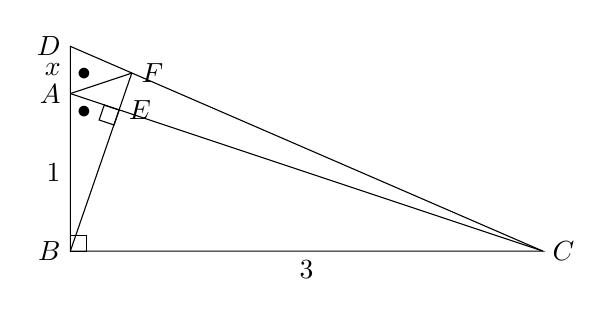
\begin{tikzpicture}
        \coordinate (A) at (0,2);
        \coordinate (B) at (0,0);
        \coordinate (C) at (6,0);
        \coordinate (D) at (0,2.6);
        \coordinate (E) at (0.62, 1.79);
        \coordinate (F) at (0.78, 2.26);
        \coordinate (G) at (0.9,2.6);
        \coordinate (H) at (1.8, 2.6);
        \coordinate (I) at (-6,0);

        \draw (D) -- (B) -- (C) -- cycle;
        \draw (A) -- (C);
        \draw (B) -- (F);
        \draw (A) -- (F);

        \node[left] at (A) {$A$};
        \node[left] at (B) {$B$};
        \node[right] at (C) {$C$};
        \node[left] at (D) {$D$};
        \node[right] at (E) {$E$};
        \node[right] at (F) {$F$};
        
        \node[left] at ($(A)!0.5!(B)$) {$1$};
        \node[below] at ($(B)!0.5!(C)$) {$3$};
        \node[left] at ($(A)!0.5!(D)$) {$x$};

        \draw pic["$\bullet$"] {angle=F--A--D};
        \draw pic["$\bullet$"] {angle=B--A--C};
        \tkzMarkRightAngle[size=.2](A,B,C);
        \tkzMarkRightAngle[size=.2](A,E,B);
    \end{tikzpicture}
\end{center}
An impulse to extend $BF$ is created. Different extension lines could be drawn to use similar triangles.
\begin{center}
    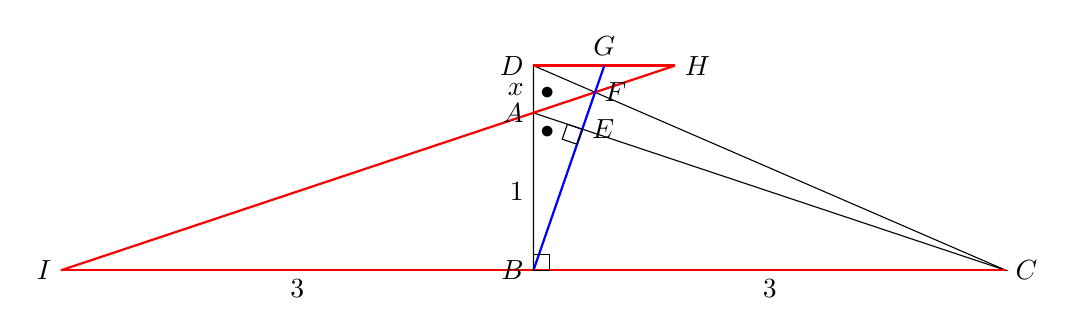
\begin{tikzpicture}
        \coordinate (A) at (0,2);
        \coordinate (B) at (0,0);
        \coordinate (C) at (6,0);
        \coordinate (D) at (0,2.6);
        \coordinate (E) at (0.62, 1.79);
        \coordinate (F) at (0.78, 2.26);
        \coordinate (G) at (0.9,2.6);
        \coordinate (H) at (1.8, 2.6);
        \coordinate (I) at (-6,0);

        \draw (D) -- (B) -- (C) -- cycle;
        \draw (A) -- (C);
        \draw (B) -- (F);
        \draw (A) -- (F);
        \draw[color=red, thick] (I) -- (H);
        \draw[color=red, thick] (I) -- (C);
        \draw[color=red, thick] (D) -- (H);
        \draw[color=blue, thick] (B) -- (G);

        \node[left] at (A) {$A$};
        \node[left] at (B) {$B$};
        \node[right] at (C) {$C$};
        \node[left] at (D) {$D$};
        \node[right] at (E) {$E$};
        \node[right] at (F) {$F$};
        \node[above] at (G) {$G$};
        \node[right] at (H) {$H$};
        \node[left] at (I) {$I$};
        
        \node[left] at ($(A)!0.5!(B)$) {$1$};
        \node[below] at ($(B)!0.5!(C)$) {$3$};
        \node[left] at ($(A)!0.5!(D)$) {$x$};
        \node[below] at ($(I)!0.5!(B)$) {$3$};

        \draw pic["$\bullet$"] {angle=F--A--D};
        \draw pic["$\bullet$"] {angle=B--A--C};
        \tkzMarkRightAngle[size=.2](A,B,C);
        \tkzMarkRightAngle[size=.2](A,E,B);
    \end{tikzpicture}
\end{center}
Looking carefully at the diagram, it could be inferred that $DG=GH$. The reason is because $\triangle{DFS}\sim\triangle{CFI}$ and $IB=BC$. In another words, $DG=\frac{3x}{2}$. Using the similar triangles again, $\frac{3x}{2}:x+1=1:3$ is true. Therefore, $x=\boxed{\frac{2}{7}}$.
\end{solution}

\section*{2021 AMC 12A Problem 12}
All the roots of the polynomial $z^6-10z^5+Az^4+Bz^3+Cz^2+Dz+16$ are positive integers, possibly repeated. What is the value of $B$?
\\\\
$\textbf{(A) }{-}88 \qquad \textbf{(B) }{-}80 \qquad \textbf{(C) }{-}64 \qquad \textbf{(D) }{-}41\qquad \textbf{(E) }{-}40$
\begin{solution}
\\\\
\textbf{Key Word} Vieta's Formula
\\\\
Using Vieta's formula, it is true that $r_1+r_2+r_3+r_4+r_5+r_6=10$ and $r_1r_2r_3r_4r_5r_6=16$. Moreover, $r_1r_2r_3+\dots+r_4r_5r_6$ is the value that needs to be computed. Remember.. all roots are positive integers!! Thus, WLOG, $r_1=1,r_2=1,r_3=2r_4=2,r_5=2\text{ and }r_6=2$.
\\\\
Now, let's be smart. The number of cases of choosing $2,2,2$ is ${}_4C_3$. Moreover, the number of cases of selecting $2,2,1$ is ${}_4C_2\cdot{}_2C_1$. Furthermore, the number of cases of choosing $2,1,1$ is ${}_4C_1\cdot{}_2C_2$. Therefore, $8\cdot{}_4C_3+4\cdot{}_4C_2\cdot{}_2C_1+2\cdot{}_4C_1\cdot{}_2C_2=32+48+8=88$. We now need to change the sign, since we used Vieta's Formula. Thus, the answer is $\boxed{\textbf{(A) }{-}88}$.
\end{solution}

\section*{2021 AMC 12A Problem 22}
Suppose that the roots of the polynomial $P(x)=x^3+ax^2+bx+c$ are $\cos \frac{2\pi}7,\cos \frac{4\pi}7,$ and $\cos \frac{6\pi}7$, where angles are in radians. What is $abc$?
\\\\
$\textbf{(A) }{-}\frac{3}{49} \qquad \textbf{(B) }{-}\frac{1}{28} \qquad \textbf{(C) }\frac{\sqrt[3]7}{64} \qquad \textbf{(D) }\frac{1}{32}\qquad \textbf{(E) }\frac{1}{28}$
\begin{solution}
\\\\
\textbf{Key Word} Vieta's Formula, The Roots of Unity, Euler's Formula, Trigonometric Identities
\\\\
First and foremost, using the Vieta's Formula, it is evident that
\begin{align*}
-a&=\cos\frac{2\pi}{7}+\cos\frac{4\pi}{7}+\cos\frac{6\pi}{7} \\
b&=\cos\frac{2\pi}{7}\cos\frac{4\pi}{7}+\cos\frac{2\pi}{7}\cos\frac{6\pi}{7}+\cos\frac{4\pi}{7}\cos\frac{6\pi}{7} \\
-c&=\cos\frac{2\pi}{7}\cos\frac{4\pi}{7}\cos\frac{6\pi}{7}
\end{align*}
\textbf{Calculating $a$} \\
Using the $7^{\text{th}}$ roots of unity, we could know that
\[
e^{2\pi\cdot\frac{0}{7}}+e^{2\pi\cdot\frac{1}{7}}+\dots+e^{2\pi\cdot\frac{5}{7}}+e^{2\pi\cdot\frac{6}{7}}
\]
is true. Moreover, using the Euler's Formula $e^{i\theta}=\cos\theta+i\sin\theta$, it is evident that the following is true.
\[
\cos\left(2\pi\cdot\frac{0}{7}\right)+\dots+\cos\left(2\pi\cdot\frac{6}{7}\right)+i\left(\sin\left(2\pi\cdot\frac{0}{7}\right)+\dots+\sin\left(2\pi\cdot\frac{6}{7}\right)\right)=0
\]
Using the trigonometric identities, the following equation may be modified.
\[
1+2\left(\cos\left(2\pi\cdot\frac{1}{7}\right)+\cos\left(2\pi\cdot\frac{2}{7}\right)+\cos\left(2\pi\cdot\frac{3}{7}\right)\right)=0
\]
In another words, $2(-a)=-1$ and $a=\frac{1}{2}$.
\\\\
\textbf{Calculating $b$} \\
The trigonometric identity $\cos\alpha\cos\beta=\frac{1}{2}(\cos(\alpha+\beta)+\cos(\alpha-\beta))$ could be used.
\begin{align*}
    b&=\frac{1}{2}\left(\cos\frac{6\pi}{7}+\cos\frac{2\pi}{7}\right)+\frac{1}{2}\left(\cos\frac{8\pi}{7}+\cos\frac{4\pi}{7}\right)+\frac{1}{2}\left(\cos\frac{10\pi}{7}+\cos\frac{2\pi}{7}\right) \\
    &=\frac{1}{2}\left(2\cos\frac{2\pi}{7}+\cos\frac{6\pi}{7}+\cos\frac{8\pi}{7}+\cos\frac{4\pi}{7}+\cos\frac{10\pi}{7}\right) \\
    &=\cos\frac{2\pi}{7}+\cos\frac{6\pi}{7}+\cos\frac{4\pi}{7} \\
    &=-a \\
    &=-\frac{1}{2}
\end{align*}

\textbf{Calculating $c$} \\
\begin{align*}
    -c=\frac{1}{2}\left(\cos\frac{6\pi}{7}+\cos\frac{2\pi}{7}\right)\left(\cos\frac{6\pi}{7}\right)&=\left(\cos\frac{6\pi}{7}+\cos\frac{2\pi}{7}+\cos\frac{6\pi}{7}\right) \\
    &=\frac{1}{2}\left(\frac{1}{2}\left(\cos\frac{12\pi}{7}+\cos\frac{0\pi}{7}\right)+\frac{1}{2}\left(\cos\frac{8\pi}{7}+\cos\frac{4\pi}{7}\right)\right) \\
    &=\frac{1}{4}\left(1+\cos\frac{12\pi}{7}+\cos\frac{4\pi}{7}+\cos\frac{8\pi}{7}\right) \\
    &=\frac{1}{4}(1-a) \\
    &=\frac{1}{8}
\end{align*}
\\\\
\textbf{Final Calculation}
\[
abc=\frac{1}{2}\left(-\frac{1}{2}\right)\left(-\frac{1}{8}\right)=\boxed{\textbf{(D) }\frac{1}{32}}
\]
\end{solution}

\end{document}
